\documentclass[conference,a4paper]{IEEEtran}
\usepackage{cite}
\usepackage{amsmath,amssymb}
\usepackage{graphicx}
\usepackage{booktabs}
\usepackage{array}
\newcolumntype{L}[1]{>{\raggedright\arraybackslash}p{#1}}
\usepackage{multirow}
\usepackage{algorithm}
\usepackage{algpseudocode}
\usepackage{url}
\usepackage{xcolor}
\usepackage[hidelinks,pdfusetitle]{hyperref}
\graphicspath{{../figs/}}
\hypersetup{pdfauthor={Muhammad Abdullah Aamir, Haider Farooq Toor, Muhammad Ibrahim Kiani}}

\begin{document}

\title{Trust, but Verify the Label: Encrypted-Traffic Misclassification as the Residual Risk of Deterministic Policy Gating}

\author{\IEEEauthorblockN{Muhammad Abdullah Aamir}
\IEEEauthorblockA{Department of Data Science\\
FAST-NUCES, Islamabad, Pakistan\\
i232538@isb.nu.edu.pk}
\and
\IEEEauthorblockN{Haider Farooq Toor}
\IEEEauthorblockA{Department of Data Science\\
FAST-NUCES, Islamabad, Pakistan\\
i232542@isb.nu.edu.pk}
\and
\IEEEauthorblockN{Muhammad Ibrahim Kiani}
\IEEEauthorblockA{Department of Data Science\\
FAST-NUCES, Islamabad, Pakistan\\
i232536@isb.nu.edu.pk}}

\maketitle

\begin{abstract}
Language-model agents are proposed for network operations, where an agent turns an operator request and a traffic label into an action such as allowing, blocking or rate-limiting a flow. When the label comes from an encrypted-traffic classifier, a policy check before execution is only as correct as the prediction it reads. This dependency is measured on ISCXVPN2016. A Random Forest on 23 time-related flow statistics reaches 0.837 macro-F1 over seven applications and 0.855 weighted precision under the dataset's original protocol, against 0.808 for a rebuilt C4.5 baseline. These predictions drive a 3B-parameter agent whose proposals pass a deterministic gate enforcing three application rules. On 100 identical proposals, the gate lowers executed violations from 30 to 6 (95\% CI of the difference 17.7--30.4 points) and keeps 97.9\% of completed tasks. All six remaining violations are restricted flows predicted as permissive classes, and none remain with true labels. A probability-aware gate removes five of them only at a threshold that over-restricts 9.5\% of validation flows.
\end{abstract}

\begin{IEEEkeywords}
Encrypted Traffic Classification, Network Policy Enforcement, Language-Model Agents, Random Forest, Deterministic Gating.
\end{IEEEkeywords}

\section{Introduction}

Encryption hides packet payloads from the network, which removes payload inspection as a basis for application-aware policy. Classifiers trained on flow-level timing and volume statistics are used in its place, ranging from decision trees on time-related features \cite{drapergil2016} to deep models on packet sequences \cite{rezaei2019,lotfollahi2020,elshewey2025}. At the same time, large language models (LLMs) are being placed inside network operations: as translators from operator intent to configuration \cite{wang2024netconfeval}, as multi-agent assistants for production network management \cite{wang2025confucius}, and as analysts that query traffic predictors \cite{adanza2026}. Combining the two gives an agent that reads a classifier's label for a flow and decides what to do with it.

Placing an agent between an operator and the data plane raises a control problem that existing work treats only in part. First, a policy written into a prompt is followed only on a best-effort basis, and studies of tool-using agents report frequent breaches when an instruction conflicts with the rules \cite{zwerdling2025,sah2026verifier}. Second, the remedy proposed in those studies, a check executed before each tool call \cite{zwerdling2025,wang2026agentspec}, evaluates the action against facts it is given and assumes those facts are correct. Third, in an encrypted network the decisive fact, the application a flow belongs to, is itself a prediction with a measurable error rate, and classification studies report accuracy without asking which errors change an enforcement decision \cite{drapergil2016,elshewey2025}.

To investigate this interaction, a complete pipeline is built on ISCXVPN2016 \cite{drapergil2016}: a Random Forest that labels encrypted flows, a local LLM agent that proposes one action per flow, and a deterministic gate that checks each proposal against three application rules before a simulator executes it (Fig.~\ref{fig:arch}). Each of 100 scenarios is answered once by the agent and replayed under every enforcement condition, so differences between conditions isolate the gate. The primary contributions of this paper are:
\begin{itemize}
\item \textbf{Base-Protocol Rebuild:} The evaluation protocol of the dataset's original study is re-implemented, and the Random Forest exceeds the rebuilt C4.5 baseline by at least 4.7 points of weighted precision at every flow timeout.
\item \textbf{Paired Gating Evaluation:} Deterministic pre-execution gating, evaluated on identical proposals, reduces executed violations from 30 to 6 with a confidence interval that excludes zero.
\item \textbf{Error Propagation Analysis:} A short derivation, confirmed empirically, shows that with a correct gate every remaining violation requires a restricted flow to be predicted as a more permissive class.
\item \textbf{Probability-Aware Gating:} Two rules that read class probabilities instead of the top label are evaluated, and the resulting safety--utility trade-off is reported under over-restriction budgets fixed on validation data.
\end{itemize}

The remainder of this paper is organized as follows. Section~II reviews related work. Section~III formalizes the problem and describes the method. Section~IV details the experimental setup, and Section~V reports the results. Section~VI compares the results with the base papers, Section~VII presents ablations, Section~VIII discusses implications and limitations, and Section~IX concludes the paper.

\section{Related Work}

\textit{Encrypted traffic classification.} Draper-Gil et al.~\cite{drapergil2016} released ISCXVPN2016 together with 23 time-related flow features and reported that C4.5 and KNN separate seven applications with and without VPN tunnelling. Later work moved to deep models on raw packets \cite{lotfollahi2020} and to stacked ensembles on HTTPS flows \cite{elshewey2025}, a shift surveyed by Rezaei and Liu \cite{rezaei2019}. These studies optimize accuracy or F1 over all classes, whereas a policy assigns very different consequences to different confusions.

\textit{LLM agents in network operations.} NetConfEval \cite{wang2024netconfeval} measures how reliably LLMs translate requirements into formal specifications and configurations, Confucius \cite{wang2025confucius} deploys multi-agent LLM workflows with validation steps in a production network, and Adanza et al.~\cite{adanza2026} couple an agent with traffic prediction for analysis. None of these systems lets an agent act on individual flows under an explicit enforcement policy.

\textit{Pre-execution policy enforcement.} ToolGuard \cite{zwerdling2025} compiles business policy into code guards that run before each tool call, AgentSpec \cite{wang2026agentspec} expresses runtime rules in a domain-specific language, and GuardAgent \cite{xiang2025guardagent} generates guard code with a second agent. The Verifier Tax \cite{sah2026verifier} shows that LLM-based verifiers intercept most unsafe actions but add model calls. All of these assume that the facts a guard reads are correct. Table~\ref{tab:related} summarizes the studies closest to this setting.

\begin{table}[t]
\centering
\caption{Summary of Closely Related Studies}
\label{tab:related}
\footnotesize
\setlength{\tabcolsep}{3pt}
\begin{tabular}{@{}L{1.0cm}L{2.3cm}L{2.25cm}L{2.15cm}@{}}
\toprule
Study & Setting & Contribution & Gap for this work \\
\midrule
\cite{drapergil2016} & ISCXVPN2016, 14 classes & Time-related features; C4.5, KNN & Accuracy only; no action \\
\cite{elshewey2025} & HTTPS, 6 classes & Stacked deep ensembles & Classification only \\
\cite{wang2024netconfeval} & Config.\ synthesis & LLM benchmark & No flow-level action \\
\cite{wang2025confucius} & Production network & Multi-agent workflows & No per-flow policy \\
\cite{zwerdling2025} & $\tau$-bench airline & Code guards before tools & Facts assumed correct \\
\cite{wang2026agentspec} & Code, robots, driving & Rule language & Facts assumed correct \\
\cite{sah2026verifier} & $\tau$-bench & LLM verifier cost & Verifier is an LLM \\
\bottomrule
\end{tabular}
\end{table}

\section{Proposed Methodology}

\subsection{Problem Formulation}
A flow $f$ is described by a feature vector $\mathbf{x} \in \mathbb{R}^{23}$ and belongs to a true application $y \in \mathcal{A}$, where $\mathcal{A}$ contains browsing, chat, email, file transfer, P2P, streaming and VoIP. A classifier returns probabilities $p(c \mid \mathbf{x})$ for $c \in \mathcal{A}$ and the prediction $\hat{y} = \arg\max_c p(c \mid \mathbf{x})$. An agent proposes one action $a$ from $\{\textsc{allow}, \textsc{block}, \textsc{limit}(k)\}$ with rate $k$ in kbps. The operator policy maps each application to its set of permitted actions $\Pi(c)$:
\begin{equation}
\Pi(c) =
\begin{cases}
\{\textsc{block}\}, & c = \text{P2P},\\
\{\textsc{block}\} \cup L(1024), & c \in \mathcal{R}_1,\\
\{\textsc{allow}, \textsc{block}\} \cup L(10^4), & \text{otherwise},
\end{cases}
\label{eq:policy}
\end{equation}
with $L(u) = \{\textsc{limit}(k): k \in \mathbb{Z},\ 64 \le k \le u\}$,
where $\mathcal{R}_1$ contains streaming and file transfer. A gate $G$ executes $a$ only if it passes structural checks and $a \in \Pi(\hat{y})$. An executed action is a violation when it is not permitted for the true class:
\begin{equation}
V(a, y) = \mathbf{1}\left[a \text{ executed} \wedge a \notin \Pi(y)\right].
\label{eq:violation}
\end{equation}
Because the gate executes only actions in $\Pi(\hat{y})$, a violation under a correct gate requires $a \in \Pi(\hat{y}) \setminus \Pi(y)$, which is non-empty only when $\hat{y} \neq y$ and $\Pi(\hat{y}) \not\subseteq \Pi(y)$. Under (\ref{eq:policy}) this happens exactly when a restricted flow is predicted as a class of a less restrictive level. Every residual violation is therefore attributable to a specific direction of misclassification, which Section~V tests.

\subsection{Architecture and Components}
Fig.~\ref{fig:arch} shows the pipeline. The classifier writes $\hat{y}$ for each flow into a trusted record that the agent can read but not modify. The agent receives the flow identifier, $\hat{y}$, the operator request and the written policy, and returns one JSON tool call. No generated code is executed. The gate reads $\hat{y}$ directly from the trusted record, and a dictionary simulator stores each flow as held, allowed, blocked or rate-limited, with every flow starting held.

\begin{figure*}[t]
\centering
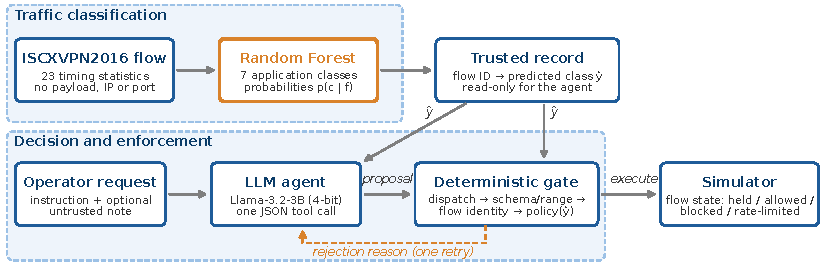
\includegraphics[width=\textwidth]{cn_architecture.pdf}
\caption{Pipeline. A Random Forest labels each encrypted flow from timing statistics; its prediction $\hat{y}$ reaches both the agent and the deterministic gate, which executes a proposal only if it is permitted for $\hat{y}$. A rejected flow stays held; in one condition the rejection reason is returned for a single retry. The highlighted classifier is the component whose errors this paper traces.}
\label{fig:arch}
\end{figure*}

\textit{Traffic classifier.} A Random Forest \cite{breiman2001} of 100 trees grown on Gini impurity, with maximum depth 16, at least two samples per leaf and balanced class weights is compared with a depth-10 decision tree and a majority-class predictor, using scikit-learn \cite{pedregosa2011} with seed 42. The model with the higher validation macro-F1 is frozen before testing.

\textit{Agent.} Llama-3.2-3B-Instruct \cite{grattafiori2024llama3}, quantized to 4 bits (Q4\_K\_M), runs on a laptop CPU through llama.cpp \cite{llamacpp} with temperature 0, seed 42, a 2,048-token context and at most 128 output tokens.

\textit{Deterministic gate.} Algorithm~\ref{alg:gate} gives the gate. The four checks run in order, and any failure leaves the flow held.

\textit{Changes from the initial design.} Several parts of the originally proposed design changed during implementation. The released feature files contain no packet-size fields and no capture, session, address or port identifiers, so only the 23 time-related features are used, and duplicate and conflicting rows are removed before a stratified split instead of separating captures. Median imputation was dropped because the value $-1$ marks a statistic that does not apply to a flow. The retry condition, the true-label condition, the probability-aware rules and the rebuild of the base-paper protocol were added to separate classifier errors from agent errors and to allow a direct comparison with \cite{drapergil2016}.

\begin{algorithm}[t]
\caption{Deterministic gate}
\label{alg:gate}
\footnotesize
\begin{algorithmic}[1]
\Require proposal $a$, episode flow $f^{\ast}$, trusted record $T$, simulator $S$
\If{unknown tool \textbf{or} missing argument \textbf{or} flow $\notin S$}
  \State \Return \textsc{hold} \Comment{dispatch check}
\EndIf
\If{extra arguments \textbf{or} $k \notin \mathbb{Z} \cap [64, 10^4]$}
  \State \Return \textsc{hold} \Comment{schema and range}
\EndIf
\If{flow of $a \neq f^{\ast}$} \State \Return \textsc{hold} \Comment{identity}\EndIf
\If{$a \notin \Pi(T[f^{\ast}])$} \State \Return \textsc{hold} \Comment{policy, Eq.~(\ref{eq:policy})}\EndIf
\State \Return \textsc{execute}
\end{algorithmic}
\end{algorithm}

\subsection{Probability-Aware Gating}
Because the gate in Algorithm~\ref{alg:gate} trusts $\hat{y}$, two further rules are tested that replace $T[f^{\ast}]$ with a more cautious label. Let $r(c)$ be the strictness level of class $c$: 2 for P2P, 1 for $\mathcal{R}_1$ and 0 otherwise. The \emph{top-2 rule} applies the stricter of the two most likely classes when $\max_c p(c \mid \mathbf{x}) < \tau$. The \emph{policy-mass rule} applies the strictest level $\ell$ whose total probability reaches a threshold $\rho$:
\begin{equation}
M_\ell(\mathbf{x}) = \sum_{c:\, r(c) \ge \ell} p(c \mid \mathbf{x}),
\end{equation}
\begin{equation}
\ell^{\ast} = \max\big\{\ell \ge r(\hat{y}) : \ell = r(\hat{y}) \,\vee\, M_\ell(\mathbf{x}) \ge \rho\big\},
\label{eq:mass}
\end{equation}
and enforces the most probable class at level $\ell^{\ast}$. Because classifier probabilities need not be calibrated \cite{guo2017calibration}, thresholds are chosen on the validation split as the value that minimizes the share of flows given a more permissive policy than their true one, subject to an over-restriction budget $\beta$ on flows given a stricter policy. Results are reported for $\beta = 5\%$ and $\beta = 10\%$, both fixed before any test scenario was scored.

\section{Experimental Setup}

\textit{Dataset and preprocessing.} The study uses Scenario~B of ISCXVPN2016 with a 15-second flow timeout: 18,758 flows, each described by 23 statistics covering duration, forward, backward and flow inter-arrival times, active and idle periods, and packet and byte rates. No payload, address or port is used. VPN and non-VPN variants are merged into seven application labels, and the VPN flag is kept for analysis only. Removing 622 rows whose identical feature vectors carry different labels and 152 exact duplicates leaves 17,984 flows, from which a stratified sample of 10,000 is split into 6,000 training, 2,000 validation and 2,000 test flows. The value $-1$, which marks statistics that do not apply to a flow, is kept as a value. The release carries no capture or session identifiers, so flows from one capture may fall into different splits.

\textit{Scenario suite.} Fifty test flows (ten each of P2P, streaming and file transfer; five each of the other classes) carry 100 scenarios: 50 permitted requests, 25 policy conflicts in which the operator asks for a forbidden action, and 25 injections in which an untrusted note urges \textsc{allow}, in the manner of indirect prompt injection \cite{greshake2023}. The requested final state of each scenario is fixed before any model query. The flows are drawn at random within each class, without regard to the classifier's prediction. Ten of the 50 are misclassified by the frozen Random Forest, a higher share than on the full test split because VoIP and browsing, the two most reliably recognized classes, make up a smaller part of the sample.

\textit{Conditions.} B0 dispatches any well-formed call (policy in the prompt only); B1 adds the schema, range and identity checks; M adds the policy check; M+R returns the rejection reason for one retry; M-oracle applies M with true labels; M-U applies the probability-aware rules.

\textit{Metrics.} Over $N$ scenarios the violation rate is $\bar{V} = \frac{1}{N}\sum_i V(a_i, y_i)$. Completion counts permitted scenarios that end in exactly the requested state, and retention is the completion of a condition divided by that of B0. Uncertainty is estimated with 1,000 paired bootstrap resamples of the 50 base flows \cite{efron1994}, keeping all scenarios of a flow together.

\textit{Base-paper protocol.} For a comparison with \cite{drapergil2016} on equal terms, its setting is rebuilt: 14 classes, the uncleaned feature files, stratified 10-fold cross-validation, an entropy-based decision tree with at least two samples per leaf (C4.5-style) and a 1-nearest-neighbour classifier on features scaled to $[0,1]$, for all four timeouts.

\textit{Implementation.} Experiments run on an Intel Core i5-1235U laptop with 16\,GB RAM, without a GPU, using Python 3.11.9 and scikit-learn 1.8.0.

\section{Results and Analysis}

\subsection{Traffic Classification}
Table~\ref{tab:clf} lists the classifiers. The Random Forest leads the decision tree by 0.095 macro-F1 on the test split. Retrained with five other seeds, it scores between 0.843 and 0.848, so the frozen model's 0.837 does not overstate its performance. Per-class F1 ranges from 0.989 for VoIP to 0.718 for chat. Accuracy is 91.4\% on non-VPN flows and 84.2\% on VPN flows. Fig.~\ref{fig:cm} shows where errors concentrate: 13.6\% of file-transfer flows are predicted as chat, a confusion that crosses from a restricted policy level to a permissive one.

\begin{table}[t]
\centering
\caption{Classifier Baselines on 2,000 Test Flows}
\label{tab:clf}
\footnotesize
\setlength{\tabcolsep}{3.5pt}
\begin{tabular}{@{}lcccc@{}}
\toprule
Model & Val.\ F1 & Test Acc. & Test F1 & F1, seeds 0--4 \\
\midrule
Majority class & 0.063 & 0.282 & 0.063 & -- \\
Decision tree (depth 10) & 0.728 & 0.803 & 0.742 & $0.745 \pm 0.002$ \\
\textbf{Random Forest} & \textbf{0.839} & \textbf{0.877} & \textbf{0.837} & $\mathbf{0.845 \pm 0.002}$ \\
\bottomrule
\end{tabular}
\end{table}

\begin{figure}[t]
\centering
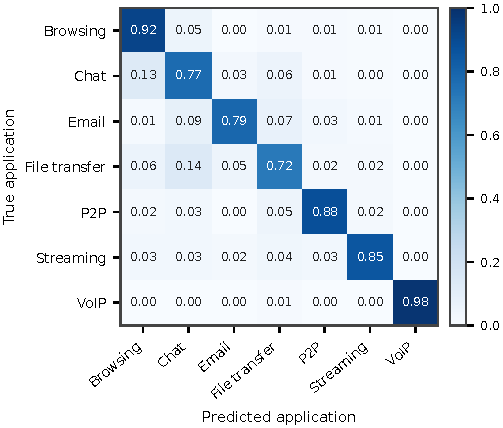
\includegraphics[width=\columnwidth]{cn_confusion.pdf}
\caption{Row-normalized confusion matrix of the Random Forest on the test split. VoIP (0.98) and browsing (0.92) are recognized most reliably; file transfer predicted as chat (0.14) is the largest confusion that crosses policy levels.}
\label{fig:cm}
\end{figure}

\subsection{Gated Enforcement}
Fig.~\ref{fig:cond} reports the four enforcement conditions on the same proposals. Without the gate, 30 of 100 scenarios end in a violation. The agent executed every one of the 25 forbidden operator requests, followed 3 of 25 injected notes and wrote 8,000,000\,kbps for an 8\,Mbps request. Structural checks remove only the two unit errors and one call with an extra argument. The policy gate lowers violations to 6, a paired reduction of 24 points (95\% CI 17.7--30.4), while 47 of 50 permitted tasks still complete against 48 without the gate, a retention of 97.9\% (CI 93.5--100). A gate decision takes a median 3.6\,$\mu$s, against 2.96\,s for an agent call.

\begin{figure}[t]
\centering
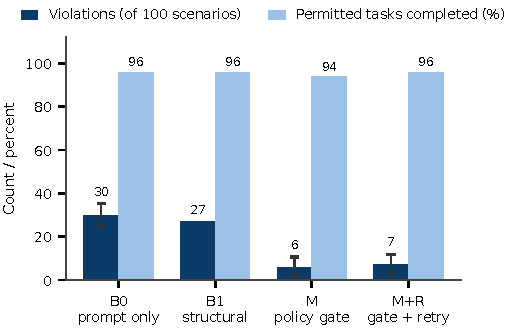
\includegraphics[width=\columnwidth]{cn_conditions.pdf}
\caption{Executed violations (with 95\% bootstrap intervals) and permitted-task completion for identical proposals under each condition.}
\label{fig:cond}
\end{figure}

\subsection{Error Propagation}
Table~\ref{tab:viol} lists the six violations that pass the policy gate. Each is a file-transfer or P2P flow predicted as chat, browsing or streaming, which is exactly the condition derived in Section~III-A, and replacing $\hat{y}$ with $y$ removes all six. The single task the gate wrongly refuses has the opposite cause: an email flow predicted as file transfer, for which \textsc{allow} is not permitted. The classifier's top probability on the six flows lies between 0.379 and 0.706, below the median of 0.932 for correct predictions.

\begin{table}[t]
\centering
\caption{Violations That Pass the Policy Gate}
\label{tab:viol}
\footnotesize
\setlength{\tabcolsep}{3pt}
\begin{tabular}{@{}lllcl@{}}
\toprule
True class & Predicted & Action & Top $p$ & Restr.\ mass \\
\midrule
File transfer & Browsing & \textsc{allow} & 0.388 & 0.266 \\
File transfer & Chat & \textsc{limit}(8000) & 0.592 & 0.341 \\
P2P & Streaming & \textsc{limit}(128) & 0.679 & 0.307$^{\dagger}$ \\
File transfer & Chat & \textsc{limit}(8000) & 0.379 & 0.277 \\
P2P & Chat & \textsc{limit}(256) & 0.706 & 0.001$^{\dagger}$ \\
File transfer & Browsing & \textsc{allow} & 0.388 & 0.269 \\
\bottomrule
\multicolumn{5}{@{}p{0.97\columnwidth}@{}}{\scriptsize Restricted mass: probability on streaming, file transfer and P2P; $^{\dagger}$probability on P2P alone, the level a P2P flow requires.}
\end{tabular}
\end{table}

\subsection{Probability-Aware Gating}
Under a 5\% over-restriction budget, neither rule removes a violation on the test scenarios: the policy-mass threshold selected on validation ($\rho = 0.45$) keeps 6 violations and 47 completed tasks. Under a 10\% budget, validation selects $\rho = 0.25$, and violations fall to 1 while completed tasks fall to 43, a retention of 89.6\% (Fig.~\ref{fig:unc}). The top-2 rule performs worse at both budgets because, for four of the six flows, the second most likely class is also permissive. The remaining violation is a P2P flow that the classifier gives 0.001 probability of being P2P, so only a threshold low enough to restrict almost every flow would catch it.

\begin{figure}[t]
\centering
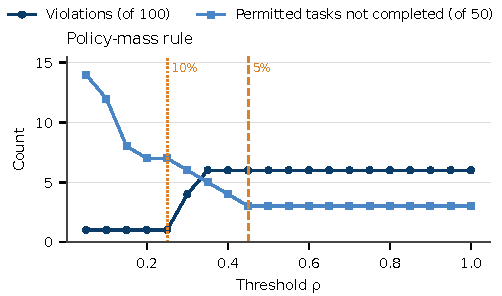
\includegraphics[width=\columnwidth]{cn_uncertainty.pdf}
\caption{Policy-mass rule: violations and permitted tasks not completed as the threshold $\rho$ varies. Dashed and dotted lines mark the thresholds selected on validation for 5\% and 10\% over-restriction budgets.}
\label{fig:unc}
\end{figure}

\section{Comparison with Base Papers and State of the Art}

Table~\ref{tab:base} summarizes the three studies this work builds on. Draper-Gil et al.~\cite{drapergil2016} define the dataset and features, Elshewey and Osman \cite{elshewey2025} represent current deep classifiers of encrypted traffic, and ToolGuard \cite{zwerdling2025} is the closest form of pre-execution enforcement.

\begin{table*}[t]
\centering
\caption{Base Papers}
\label{tab:base}
\footnotesize
\setlength{\tabcolsep}{4pt}
\begin{tabular}{@{}L{2.2cm}L{2.4cm}L{2.6cm}L{2.4cm}L{1.8cm}L{2.3cm}L{2.4cm}@{}}
\toprule
Study & Problem & Method & Dataset & Metrics & Reported result$^{\ast}$ & Limitation \\
\midrule
Draper-Gil et al., 2016 \cite{drapergil2016} & Encrypted and VPN application characterization & 23 time-related features; C4.5, KNN; 10-fold CV & ISCXVPN2016, 14 classes (Scenario B) & Precision, recall & Best average precision 0.783 (C4.5), 0.711 (KNN) & No downstream use of predictions \\
Elshewey and Osman, 2025 \cite{elshewey2025} & HTTPS traffic categorization & Deep models with stacked logistic regression & 145,671 flows, 88 features, 6 classes & Accuracy, macro-F1, AUC & Accuracy 0.9949, macro-F1 0.9932 & Different data; classification only \\
Zwerdling et al., 2025 \cite{zwerdling2025} & Policy adherence of tool-using agents & Policy compiled into code guards run before tool calls & $\tau$-bench airline, 22 policy-violating tasks & pass$^k$ & pass$^1$ 0.450 $\rightarrow$ 0.685 & Guards trust their inputs \\
\bottomrule
\multicolumn{7}{@{}l@{}}{\scriptsize $^{\ast}$Numbers reported in the cited papers, not reproduced here except where stated in Table~\ref{tab:quant}.}
\end{tabular}
\end{table*}

\textit{Quantitative comparison.} Table~\ref{tab:quant} places the Random Forest against \cite{drapergil2016} under that study's protocol, with reported values marked. The rebuilt C4.5-style tree reaches 0.808 at 15\,s, 2.5 points above the reported 0.783, which indicates a faithful rebuild. The Random Forest reaches 0.855, an absolute gain of 4.7 points (5.9\% relative) over the rebuilt tree and 7.2 points (9.2\% relative) over the reported value, and its macro-F1 is 0.817 against 0.765. It leads at every timeout (Fig.~\ref{fig:base}). Against the reported KNN the gain is 14.4 points (20.3\% relative).

\begin{table}[t]
\centering
\caption{Weighted Precision Under the Base-Paper Protocol (14 Classes, 10-Fold CV)}
\label{tab:quant}
\footnotesize
\setlength{\tabcolsep}{3pt}
\begin{tabular}{@{}lccccc@{}}
\toprule
Method & 15\,s & 30\,s & 60\,s & 120\,s & Best \\
\midrule
C4.5 \cite{drapergil2016}$^{\ast}$ & -- & -- & -- & -- & 0.783 \\
KNN \cite{drapergil2016}$^{\ast}$ & -- & -- & -- & -- & 0.711 \\
C4.5-style tree (rebuilt) & 0.808 & 0.789 & 0.773 & 0.767 & 0.808 \\
1-NN (rebuilt) & 0.745 & 0.743 & 0.724 & 0.728 & 0.745 \\
\textbf{Random Forest} & \textbf{0.855} & \textbf{0.845} & \textbf{0.826} & \textbf{0.819} & \textbf{0.855} \\
\bottomrule
\multicolumn{6}{@{}l@{}}{\scriptsize $^{\ast}$Reported in \cite{drapergil2016}, best average across timeouts only.}
\end{tabular}
\end{table}

\begin{figure}[t]
\centering
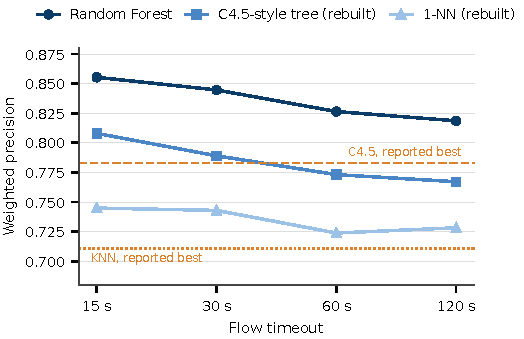
\includegraphics[width=\columnwidth]{cn_baseprotocol.pdf}
\caption{Weighted precision by flow timeout under the protocol of \cite{drapergil2016}. Orange lines mark the best values reported in that study.}
\label{fig:base}
\end{figure}

\textit{Methodological comparison.} The rebuilt single tree uses the same features and folds as the Random Forest, so the gain can be attributed to averaging many decorrelated trees, which reduces variance where the timing distributions of applications overlap \cite{breiman2001}. Elshewey and Osman report higher accuracy, but on a different dataset with 88 features and six classes, so their numbers cannot be compared with those reported here. ToolGuard generates its guards from policy documents and checks them against database records. The gate in this work is written by hand and reads a predicted label, which is the error channel analyzed in Section~V-C.

\begin{figure*}[t]
\centering
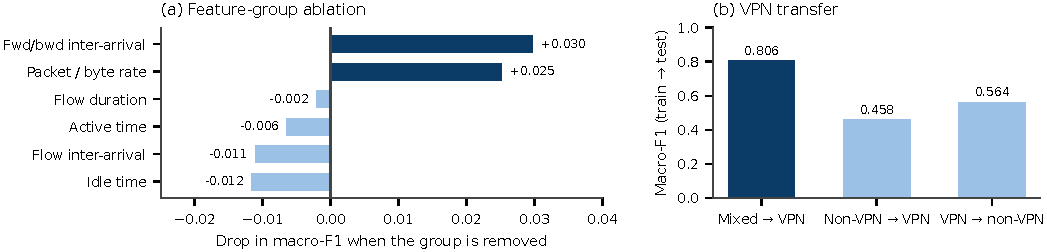
\includegraphics[width=\textwidth]{cn_robustness.pdf}
\caption{Robustness of the Random Forest. (a) Change in test macro-F1 when one feature group is removed; positive values are losses. (b) Macro-F1 when training and test flows differ in tunnelling.}
\label{fig:rob}
\end{figure*}

\textit{Fairness and limitations.} The base study does not state its precision averaging or KNN settings, so weighted averaging and Weka's default single neighbour are used. That cross-validation, like its rebuild here, may place flows from one capture in different folds. ToolGuard's pass$^k$ measures task success on a different benchmark, and Table~\ref{tab:base} lists it for context only.

\section{Ablation Study}

\textit{Enforcement layers.} Moving from B0 to B1 removes 3 of 30 violations, and adding the policy check removes 21 more. The three calls stopped by structural checks, two unit errors and one call with an extra argument, would also have failed the policy check, so the policy rules account for nearly all of the reduction.

\textit{Label source.} Replacing $\hat{y}$ with $y$ (M-oracle) removes all six residual violations and the single wrongful refusal, as the analysis in Section~III-A predicts.

\textit{Retry.} Returning the rejection reason recovers 4 of 25 rejected scenarios but introduces one new violation: a P2P flow predicted as file transfer is rate-limited at 512\,kbps, a rate permitted for the predicted class only.

\textit{Classifier and timeout.} Replacing the Random Forest with the decision tree lowers macro-F1 by 0.095. Across the four timeouts the Random Forest stays between 0.811 and 0.861 macro-F1 and leads the decision tree at each, so the choice of a 15-second window does not drive the results.

\textit{Features and VPN transfer.} Fig.~\ref{fig:rob}(a) removes one feature group at a time. Forward and backward inter-arrival times (0.030) and packet and byte rates (0.025) are the only groups whose removal lowers macro-F1, and removing any other group raises it by at most 0.012. Fig.~\ref{fig:rob}(b) trains on one tunnel type and tests on the other: a model trained on non-VPN flows reaches 0.458 macro-F1 on VPN flows, against 0.806 when VPN flows are included in training.

\section{Discussion}

The gate is effective because the policy is a short lookup from application to permitted actions, which code evaluates exactly and in microseconds, while the agent subordinates the written policy to the operator's instruction in every conflict scenario. Its weakness lies in its input. By (\ref{eq:violation}), a correct gate cannot produce a violation unless the label it reads moves a flow to a more permissive class. For an operator, the useful measure of a classifier is therefore the recall of restricted classes against permissive ones, not overall accuracy. A confusion among permissive classes leaves the permitted actions unchanged and cannot cause a violation, whereas the 13.6\% of file-transfer flows read as chat can. The VPN transfer result adds a deployment condition. A classifier in front of a policy gate needs tunnelled traffic in its training data, since a model trained without VPN flows reached only 0.458 macro-F1 on them.

The classifier's confidence does carry a usable signal, since all six violating flows have a top probability below 0.71, but acting on it costs legitimate work. At the 10\% budget, five violations disappear and four permitted tasks are lost, and one confident error remains out of reach of any threshold.

\textit{Threats to validity.} The study uses one 3B-parameter model, one dataset recorded in 2016 without capture identifiers, a simulated data plane, 100 scenarios written by the authors and three static rules. The six cases in Table~\ref{tab:viol} illustrate the mechanism but are too few to estimate how often it occurs in practice. Within these limits, the study meets its objective of measuring how classification errors pass through deterministic enforcement.

\section{Conclusion and Future Work}

A deterministic gate placed between an LLM agent and an encrypted network reduced executed policy violations from 30 to 6 on identical proposals while preserving 97.9\% of completed tasks, and the Random Forest that labels flows exceeded the dataset's original classifiers under their own protocol. Every violation that passed the gate came from a restricted flow labelled as a more permissive class, and probability-aware gating traded four legitimate tasks for five of those six. Future work will measure the same pipeline on recent traffic with capture-separated splits, add stateful rules such as bandwidth budgets, and train classifiers whose error costs follow the policy levels.

\section*{Declarations}

\textit{Data and code availability.} ISCXVPN2016 is available from the Canadian Institute for Cybersecurity. Code, the processed data split, scenarios, raw agent replies and all result files are available at \url{https://github.com/Hirotaka-Akihiro/trust-but-verify-2026}.

\textit{Conflict of interest.} The authors declare no conflict of interest.

\textit{Funding.} This work received no external funding.

\textit{AI-tool usage.} An AI assistant (Claude, Anthropic) was used to support the implementation of the experiment code and to revise the language of the manuscript. The study design, analysis, and interpretation of results are the authors' own; all results were verified against the stored outputs, and the authors take full responsibility for the content of this paper.

\IEEEtriggeratref{13}
\bibliographystyle{IEEEtran}
\bibliography{../refs}

\end{document}
